\documentclass[10pt]{article}
\usepackage[margin=1in]{geometry}

\usepackage[shortlabels]{enumitem}
\setcounter{secnumdepth}{4}


\usepackage{mathptmx}
\usepackage{graphicx}
\usepackage{times}
\usepackage{comment}
\usepackage{amstext}
\usepackage{amsmath}
\usepackage{amssymb}
\usepackage{array}
\usepackage{multirow}
\usepackage{url}
\usepackage{subfigure}
\usepackage{xcolor}
\usepackage{float}
\usepackage{slashbox}
\usepackage{pict2e}


\usepackage{fancyhdr, lastpage}
\pagestyle{fancy}
\fancyhf{}
%
\lhead{}
\chead{Simulated volume data}
\rhead{}
%
\cfoot{Page \thepage{} of \protect\pageref*{LastPage}}

\usepackage{varioref}
\labelformat{equation}{(#1)}

% \usepackage{hyperref} must almost always be LAST \usepackage in
% preamble. Otherwise, you may get strange compilation errors!
\usepackage[colorlinks,linkcolor=black]{hyperref}

\begin{document}
\section{Clean DWI (b-value=1500, SNR=10000)}
\begin{figure}[H]
  \centering
  \includegraphics[width=0.75\textwidth]{figures/DWI01.eps}
\end{figure}
\begin{figure}[H]
  \centering
  \includegraphics[width=0.75\textwidth]{figures/DWI02.eps}
\end{figure}
\begin{figure}[H]
  \centering
  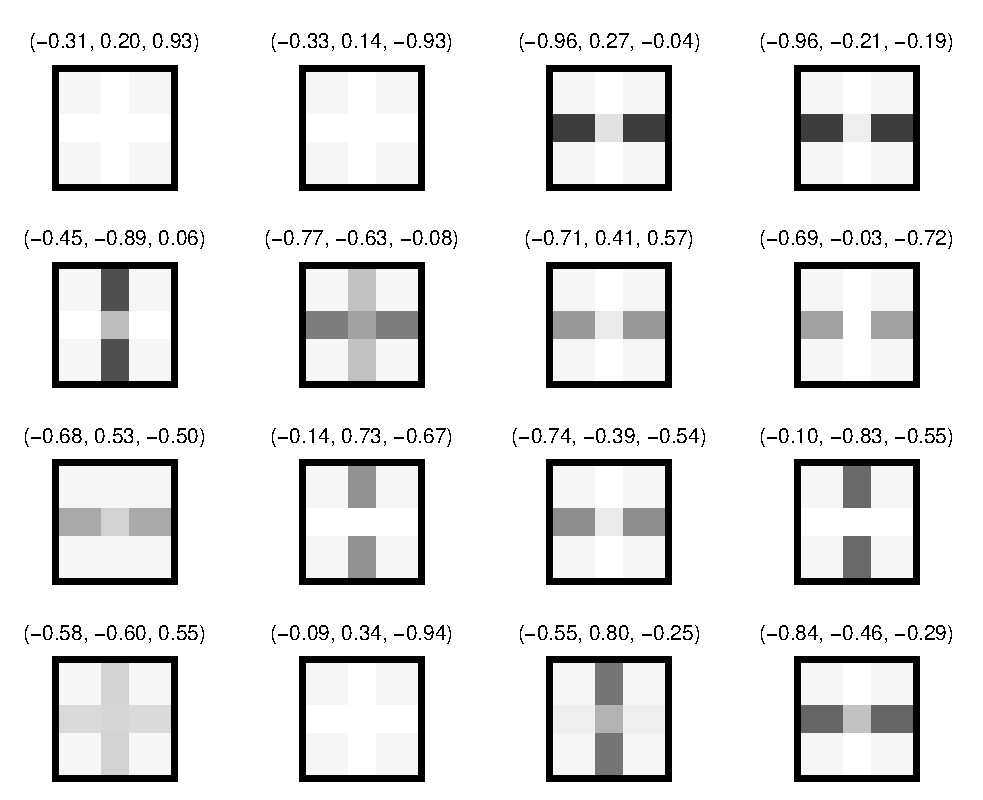
\includegraphics[width=0.75\textwidth]{figures/DWI03.eps}
\end{figure}
\begin{figure}[H]
  \centering
  \includegraphics[width=0.75\textwidth]{figures/DWI04.eps}
\end{figure}
\begin{figure}[H]
  \centering
  \includegraphics[width=\textwidth]{figures/ODF[SNR=10000].eps}
  \caption{Clean ODFs}
\end{figure}

\clearpage

\section{Noisy DWI (b-value=1500, SNR=10)}
\begin{figure}[H]
  \centering
  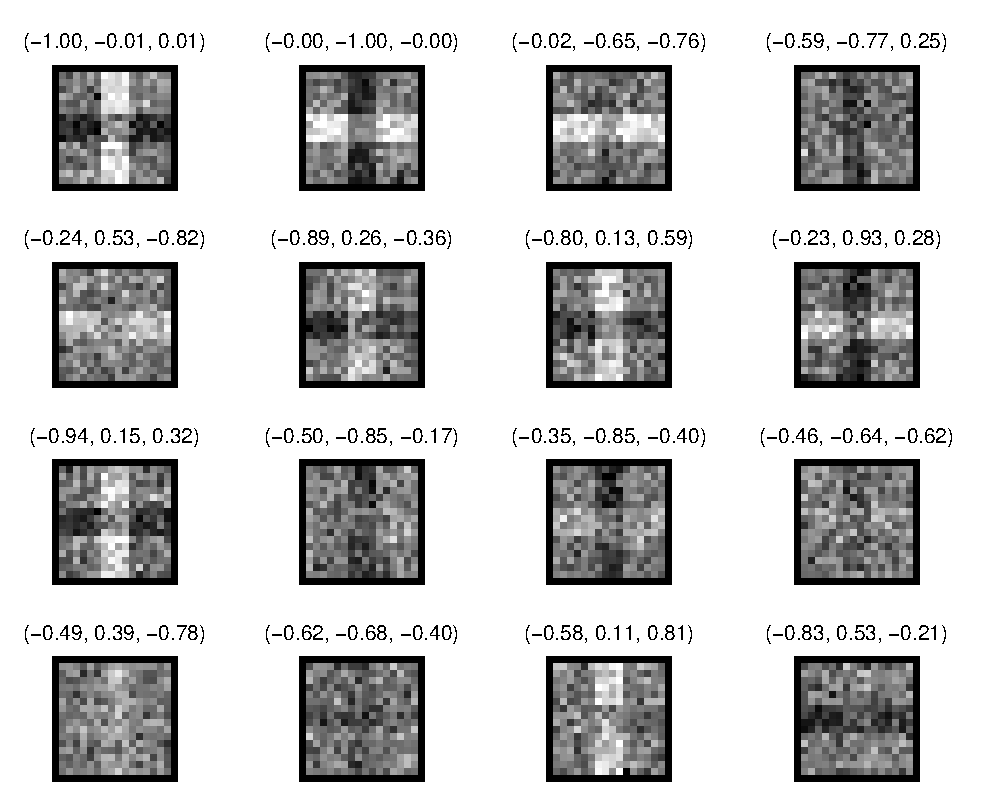
\includegraphics[width=0.75\textwidth]{figures/DWI01[SNR=10].eps}
\end{figure}
\begin{figure}[H]
  \centering
  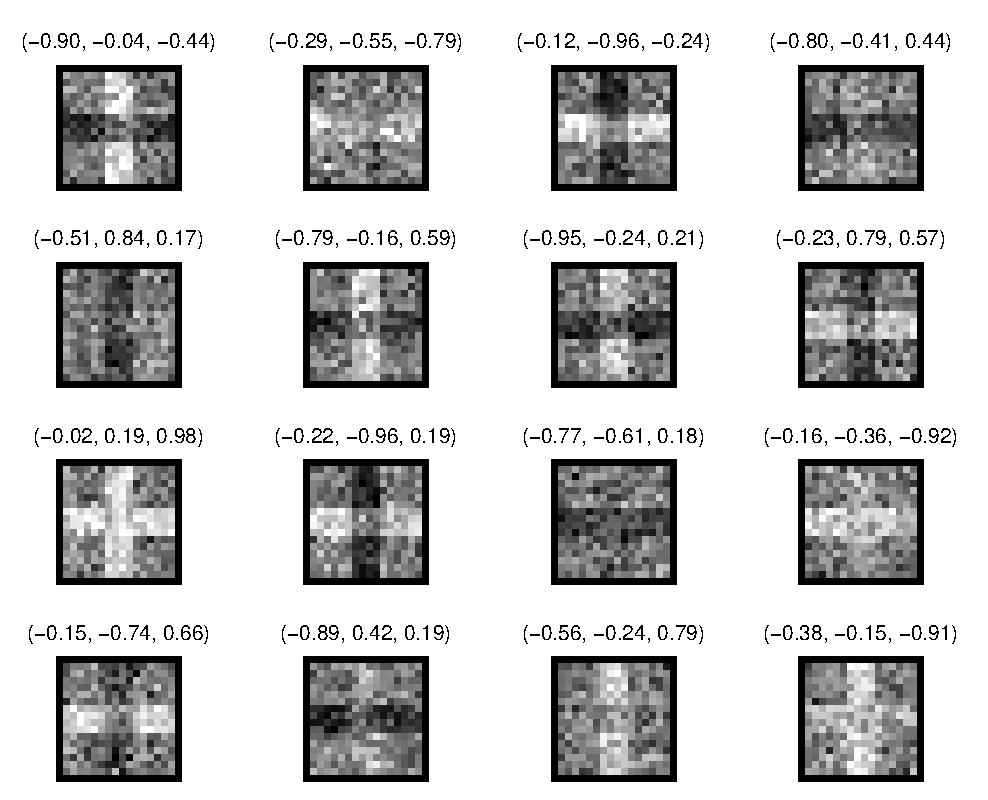
\includegraphics[width=0.75\textwidth]{figures/DWI02[SNR=10].eps}
\end{figure}
\begin{figure}[H]
  \centering
  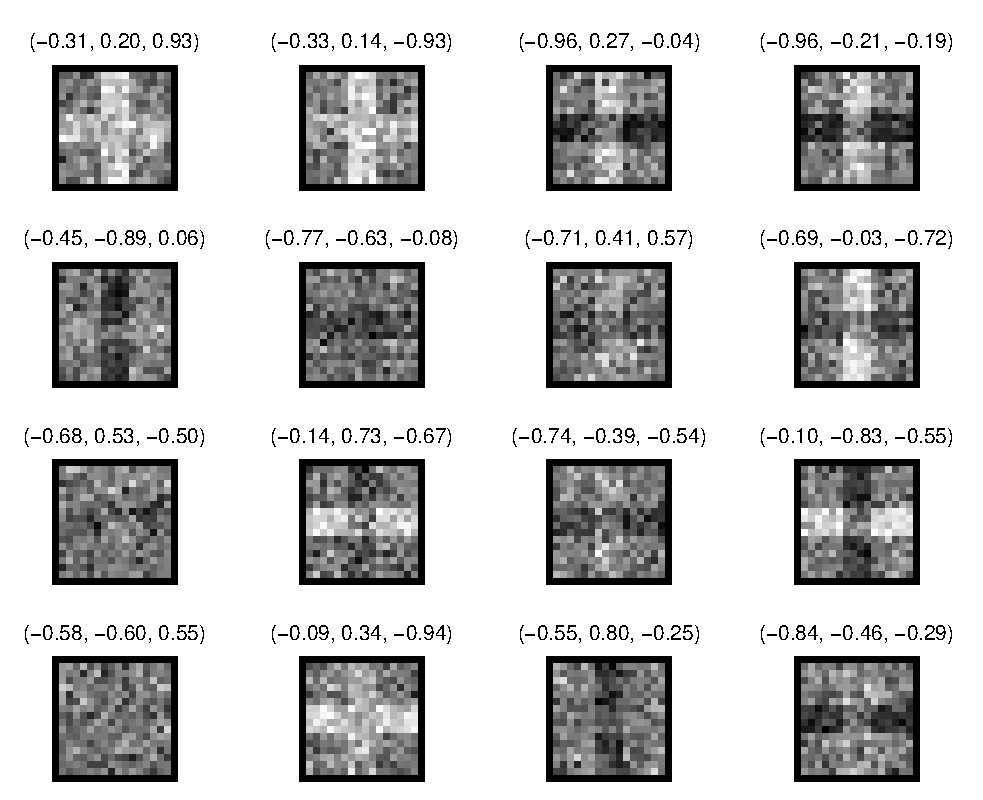
\includegraphics[width=0.75\textwidth]{figures/DWI03[SNR=10].eps}
\end{figure}
\begin{figure}[H]
  \centering
  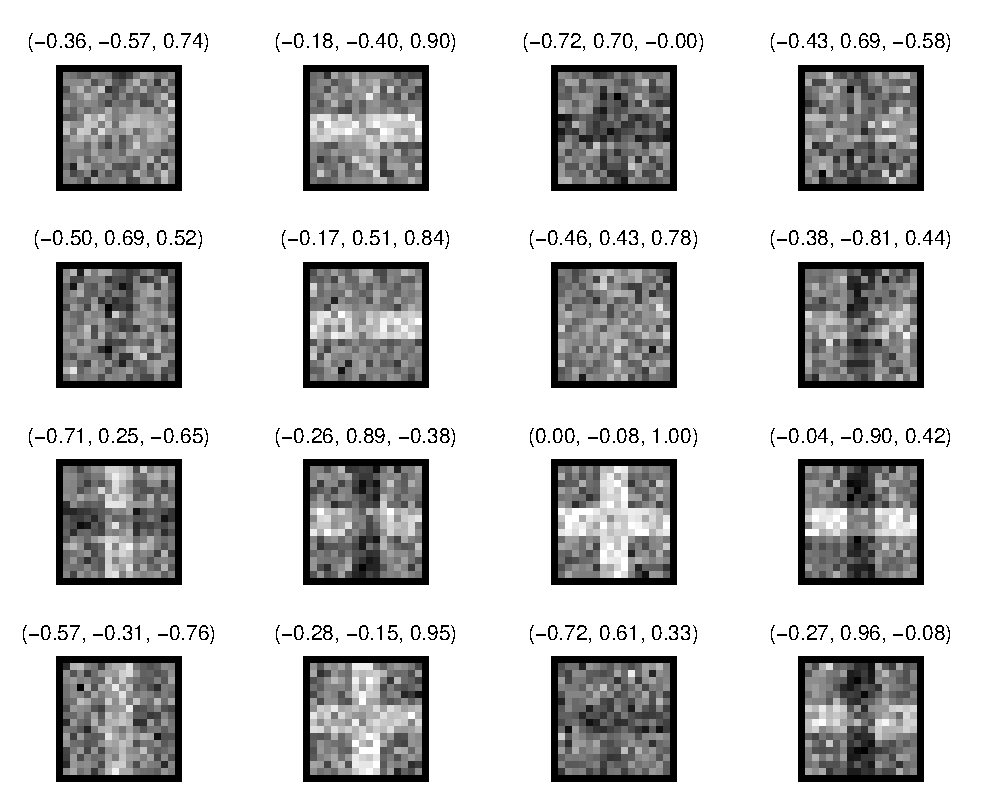
\includegraphics[width=0.75\textwidth]{figures/DWI04[SNR=10].eps}
\end{figure}
\begin{figure}[H]
  \centering
  \includegraphics[width=\textwidth]{figures/ODF[SNR=10].eps}
  \caption{Noisy ODFs}
\end{figure}
\end{document}


